\chapter{Detecção facial com OpenCV}\label{cap:opencv}

%\chapterprecis{Detecção facial utilizando a biblioteca OpenCV.}

OpenCV (Open Source Computer Vision Library) é uma biblioteca multiplataforma de código aberto (licença BSD) voltada principalmente para aplicações de visão computacional em tempo real \cite{kaehler2016learning}. Ela foi lançada oficialmente em 1999 pela Intel Corporation e continua em constante desenvolvimento.
Apesar de ser escrita em C e C++, existem interfaces em diversas outras linguagens, como Python, Java e MATLAB.

\section{Bases de faces para treino e testes}\label{sec:banco_faces}

Existe uma grande quantidade de bancos de imagens de faces disponíveis para treinar e testar algoritmos de detecção e reconhecimento facial, cada uma com características próprias \cite{grgic2013face, huang2007labeled, mozaffari2011twins}. A \autoref{tab:banco_faces} lista alguns deles.

\begin{longtabu} to \textwidth { >{\footnotesize}X[3,l] >{\footnotesize}X[1,l] >{\footnotesize}X[1,l] >{\footnotesize}X[3,l] }
\caption{Bancos de imagens de faces}
\label{tab:banco_faces}\\
\textbf{Banco de imagens}                                                            & \textbf{Indivíduos}  & \textbf{Imagens}                & \textbf{Comentários}                                                    \\\hline
\endfirsthead
\textbf{Banco de imagens}                                                            & \textbf{Indivíduos}  & \textbf{Imagens}                & \textbf{Comentários}                                                    \\\hline
\endhead
AR Face Database                                  \cite{martinez1998ar}              & 126                  & 4000                            & Pose frontal, expressão, iluminação, oclusão (óculos, cachecol)         \\\hline
AT\&T Database                                    \cite{samaria1994parameterisation} & 40                   & 400                             & Variação temporal, iluminação, expressão, óculos                        \\\hline
BANCA database                                    \cite{bailly2003banca}             & 208                  & 2496                            & Voz e face, voltado para sistemas multimodais de verificação            \\\hline
BioID Face Database                               \cite{jesorsky2001robust}          & 23                   & 1521                            & Tons de cinza, plano de fundo, iluminação, expressão, posição dos olhos \\\hline
Caltech Faces                                     \cite{weber1995caltech}            & 27                   & 450                             & Iluminação, expressão, plano de fundo                                   \\\hline
Caltech 10000 Web Faces                           \cite{angelova2005pruning}         & $\approx$ 10000      & 10000                           & Grande variedade, características faciais anotadas                      \\\hline
CAS-PEAL Face Database                            \cite{gao2008cas}                  & 1040                 & 99594                           & Expressão, acessórios, iluminação, poses múltiplas, chinês              \\\hline
CelebA                                            \cite{liu2015faceattributes}       & 10177                & 202599                          & Grande variedade, características faciais anotadas                      \\\hline
Cohn-Kanade AU-Coded Facial Expression Database   \cite{cohn1999automated}           & 100                  & 500 sequências                  & Sequência dinâmica de expressões faciais                                \\\hline
Disguise Face Database                            \cite{singh2009face}               & ?                    & ?                               & 10 variações por indivíduo usando disfarces sintéticos (barba, etc)     \\\hline
EQUINOX HID Face Database                         \cite{socolinsky2001illumination}  & 91                   & ?                               & Imagens infra vermelho, frontal                                         \\\hline
Face Video Database da Sociedade Max Planck       \cite{kleiner2004mpi}              & ?                    & 246 sequências de vídeo         & 6 pontos de vista simultâneos, vídeo                                    \\\hline
Face Recognition Grand Challenge Databases        \cite{phillips2005overview}        & > 466                & > 50000 imagens e varreduras 3D & Bem grande, iluminação, expressão, plano de fundo, 3D, sequencias       \\\hline
FEI Face Database                                 \cite{junior2006captura}           & 200                  & 2800                            & Cor, fundo branco, expressão, rotação de cabeça                         \\\hline
FERET Database (Color)                            \cite{phillips1998feret}           & 1199                 & 14126                           & Variação temporal, cor, expressão, pose e iluminação controladas        \\\hline
Georgia Tech Face Database                        \cite{georgiatechfacedatabase}     & 50                   & 750                             & Expressão, iluminação, escala, orientação                               \\\hline
Indian Face Database                              \cite{vidit2002indian}             & 40                   & > 440                           & Frontal, Índia                                                          \\\hline
Japanese Female Facial Expression                 \cite{lyons1998coding}             & 10                   & 213                             & Emoções, indivíduos femininos, Japão                                    \\\hline
Labeled Faces in the Wild                         \cite{huang2007labeled}            & 5749                 & 13233                           & Pose, iluminação, expressão, plano de fundo, diversidade                \\\hline
MIT-CBCL Face Recognition Database                \cite{weyrauch2004component}       & 10                   & > 2000                          & Imagens de modelos 3D, iluminação, pose, fundo                          \\\hline
M2VTS Multimodel Face Database (Release 1.00)     \cite{sanchez1997statistical}      & 37                   & 185                             & Grandes mudanças de pose, indivíduos falando, óculos, mudanças no tempo \\\hline
M2VTS, Extended, Univ. of Surrey, UK              \cite{messer1999xm2vtsdb}          & 295                  & 1180 vídeos                     & Rotação de cabeça, indivíduos falando, modelos 3D, alta definição       \\\hline
NIST Mugshot ID                                   \cite{watson1994nist}              & 1573                 & 3248                            & Imagens frontais e de perfil                                            \\\hline
PIE Database, CMU                                 \cite{sim2002cmu}                  & 68                   & 41368                           & Bem grande, pose, iluminação, expressão                                 \\\hline
Plastic Surgery Database                          \cite{singh2010plastic}            & 900                  & 1800                            & Imagens antes e depois de diferentes tipos de cirurgia plástica         \\\hline
Psychological Image Collection at Stirling (PICS) \cite{hancock2004psychological}    & ?                    & ?                               & Voltado para experimentos de psicologia                                 \\\hline
Synthetic Face Disguise Database                  \cite{singh2009face}               & 100                  & 4000                            & Faces sintéticas com disfarces variados                                 \\\hline
UCD Colour Face Image Database for Face Detection \cite{sharma2003colour}            & $\approx$ 299        & 299                             & Voltado para detecção, bastante variado, cor                            \\\hline
UMIST Face Database                               \cite{graham1998characterising}    & 20                   & 564                             & Pose, gênero, raça, tons de cinza                                       \\\hline
University of Essex, UK                           \cite{spacek1996university}        & 395                  & 7900                            & Diversidade racial, óculos, barbas, universitários                      \\\hline
University of Oulu Physics-Based Face Database    \cite{marszalec2000physics}        & 125                  & > 2000                          & Iluminação bastante variada, óculos                                     \\\hline
VALID Database                                    \cite{fox2005realistic}            & 106                  & 530                             & Condições de escritório altamente variáveis                             \\\hline
VidTIMIT Database                                 \cite{sanderson2008biometric}      & 43                   & Múltiplos vídeos por pessoa     & Vídeo, áudio, rotação de cabeça                                         \\\hline
Yale Face Database                                \cite{belhumeur1997eigenfaces}     & 15                   & 165                             & Tons de cinza, expressões, óculos, iluminação                           \\\hline
Yale Face Database B                              \cite{georghiades2001few}          & 10                   & 5760                            & Pose, iluminação
\end{longtabu}


Este trabalho utilizou quatro dessas bases:

\begin{description}
\item [FERET] 
É um banco de faces criado por P. Jonathon Phillips e Harry Wechsler entre 1993 e 1996 como parte do programa FERET (Facial Recognition Technology), patrocinado pelo Departamento de Defesa dos Estados Unidos.
A cópia utilizada neste trabalho foi obtida através de solicitação por email ao NIST (\textit{National Institute of Standards and Technology}).
Esta base contém 14126 imagens tiradas em condições controladas com algumas variações de ângulo e expressão.
Alguns dos indivíduos foram fotografados múltiplas vezes em diferentes anos, o que permite estudar mudanças de aparência.
Para o treino do classificador, foram selecionadas apenas 2409 fotos frontais.

\item [FEI]
É um banco de criado pelo laboratório de processamento de imagens do Centro Universitário FEI em São Bernardo do Campo. Ele é composto por 14 imagens de 200 indivíduos (100 homens e 100 mulheres), totalizando 2800 fotografias. Todas as imagens são coloridas e com fundo branco.
Para o treino do classificador, foram utilizadas 400 fotos frontais.

\item [Caltech 10000 Web Faces]
É um banco que contém 10524 faces em 7092 imagens obtidas da internet. As coordenadas dos olhos, nariz e centro da boca estão anotadas em um arquivo, o que permitiu cortar as imagens para serem usadas no treinamento do classificador. Algumas imagens foram excluídas por não mostrar suficientemente o rosto, estarem muito rotacionadas ou não possuírem resolução suficiente.

\item [LFW]
(Labeled Faces in the Wild). É um banco de 13233 imagens coletadas da internet criado e distribuído pela universidade de Massachussetts para estudar reconhecimento facial irrestrito.
Essa base foi utilizada apenas para testar o classificador.
\end{description}


\section{Treino do Classificador}\label{sec:treino_classificador}

\subsection{Imagens de treinamento}\label{sec:imagens_de_treino}

Para treinar um classificador, é preciso um conjunto de imagens positivas (imagens contendo faces) e um conjunto de imagens negativas (imagens de fundo).

\citeonline{viola2004robust} usaram 4916 imagens positivas e 9500 imagens negativas, posteriormente, \citeonline{lienhart2003empirical} concluíram que, nas condições usadas por eles, utilizar mais do que 5000 imagens positivas e 3000 imagens negativas traz pouco benefício para o resultado do treinamento.

Imagens positivas podem ser obtidas de algum banco listado na \autoref{sec:banco_faces}. Se o banco escolhido não possuir uma quantidade suficiente de exemplos, é possível aplicar transformações como rotação, inversão e alteração de intensidade às imagens existentes.

Após obter imagens positivas, é preciso identificar onde as faces estão localizadas utilizando um arquivo com formato específico, no qual cada linha contém o caminho da imagem, a quantidade de faces marcadas e coordenadas que descrevem retângulos em volta das faces.

O OpenCV possui uma ferramenta chamada \texttt{opencv\_annotation} que permite marcar com o cursor do mouse as regiões contendo faces. O comando para executá-la é \mintinline[breaklines]{bash}{opencv_annotation --annotations=/diretorio/anotacao.txt --images=/diretorio/das/imagens/}, como mostra a \autoref{fig:opencv_annotation}. 

\begin{figure}[htbp]
   \caption{Ferramenta de anotação do OpenCV}
   \label{fig:opencv_annotation}
   \begin{center}
     \scalebox{0.6}{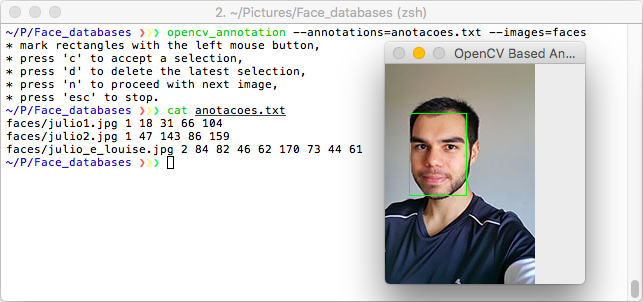
\includegraphics{imagens/opencv_annotation.png}}
   \end{center}
\end{figure}

Se as imagens contiverem apenas faces já cortadas, é possível gerar o arquivo de anotações com o comando \mintinline[breaklines]{bash}{$ find positivas/ -name "*.jpg" -exec identify -format '%i 1 0 0 %w %h\n' {} \; > anotacoes.txt}.

Também é preciso listar as imagens negativas, o que pode ser feito com o comando \mintinline[breaklines]{bash}{$ find negativas/ -name "*.jpg" > negativas.txt}.


\subsection{Treinamento}\label{sec:treinamento}

\begin{figure}[htbp]
   \caption{Criação do vetor}
   \label{fig:opencv_createsamples}
   \begin{center}
     \scalebox{0.6}{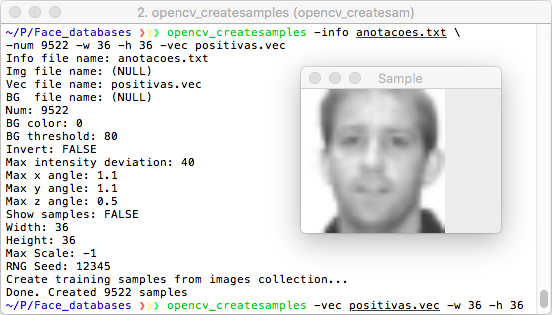
\includegraphics{imagens/opencv_createsamples.png}}
   \end{center}
\end{figure}

A OpenCV também possui ferramentas para o treinamento do classificador. 
Primeiro é necessário criar um arquivo de vetor com o comando \texttt{opencv\_createsamples}, passando a quantidade de exemplos, a largura e a altura como parâmetros. Exemplo: \mintinline[breaklines]{bash}{$ opencv_createsamples -info anotacoes.txt -num 2400 -w 24 -h 24 -vec positivas_24x24.vec}.

Para visualizar as imagens inseridas no vetor, basta usar o mesmo comando, mas passando o vetor como parâmetro: \mintinline[breaklines]{bash}{$ opencv_createsamples -vec positivas_24x24.vec -w 24 -h 24}.

Finalmente, o classificador em cascata é treinado com o comando \texttt{opencv\_traincascade}, que recebe como parâmetros um diretório onde o classificador será salvo, o arquivo de vetor gerado anteriormente, a lista de imagens negativas, a quantidade de imagens positivas e negativas, o número e estágios da cascata e as dimensões das imagens no vetor.
Exemplo: \mintinline[breaklines]{bash}{$ opencv_traincascade -data classificador/ -vec positivas_24x24.vec -bg negativas.txt -numPos 2000 -numNeg 1000 -numStages 10 -w 24 -h 24}.

\begin{figure}[htbp]
    \centering
    \caption{Treinamento do classificador em cascata usando \texttt{opencv\_traincascade}}
   \label{fig:opencv_traincascade}
    \begin{subfigure}[t]{0.49\textwidth}
    \centering
    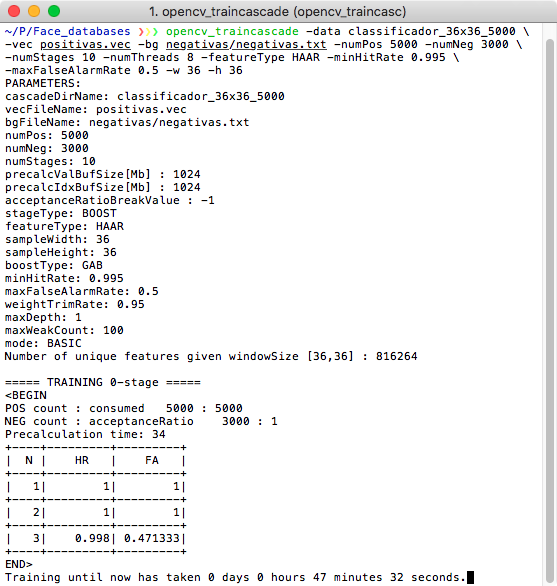
\includegraphics[width=0.95\linewidth]{imagens/opencv_traincascade_inicio.png}
    \caption{Início}\label{fig:opencv_traincascade:a}
    \end{subfigure}
    \begin{subfigure}[t]{0.49\textwidth}
    \centering
    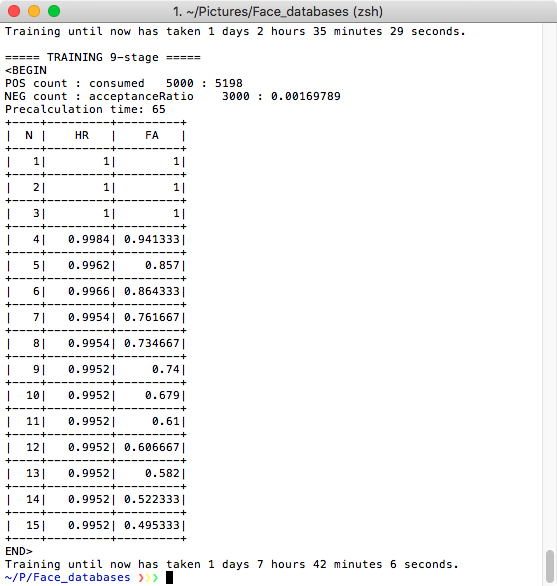
\includegraphics[width=0.95\linewidth]{imagens/opencv_traincascade_fim.png}
    \caption{Fim}\label{fig:opencv_traincascade:b}
    \end{subfigure}
\end{figure}

O treinamento pode demorar vários dias dependendo das especificações do computador e dos parâmetros passados para o comando \texttt{opencv\_traincascade}.
Como visto na \autoref{fig:opencv_traincascade}, o treinamento de um classificador em cascata de 10 estágios utilizando 5000 imagens positivas e 3000 imagens negativas com 36$\times$36 pixels cada demorou 1 dia 7 horas e 42 minutos para ser concluído em um MacBook Air de 2013 com processador Intel Core i5 de 1,3 GHz e 4 GB de RAM.


\section{Uso do classificador}\label{sec:uso_classificador}

Como resultado do treinamento, um arquivo chamado \texttt{cascade.xml} é criado no diretório especificado. Esse arquivo é o classificador em cascata treinado.
Ele pode ser carregado com o método \texttt{cv2.CascadeClassifier} do OpenCV, como usado no \autoref{cod:detector_facial_opencv}, cuja execução pode ser vista na \autoref{fig:detector_facial} e na \autoref{fig:detector_facial_lfw}.

Pela \autoref{fig:detector_facial_lfw}, é possível perceber que o classificador em cascata foi capaz de detectar faces com alguma oclusão, levemente rotacionadas e com expressões, porém o número de falso-positivos foi consideravelmente alto. Este resultado sugere que o classificador deve ser treinado com mais imagens negativas, mais estágios e com um valor menor para o parâmetro maxFalseAlarmRate.

\begin{figure}[htbp]
    \caption{Captura de tela do \autoref{cod:detector_facial_opencv} em execução.}
    \label{fig:detector_facial}
    \begin{center}
        {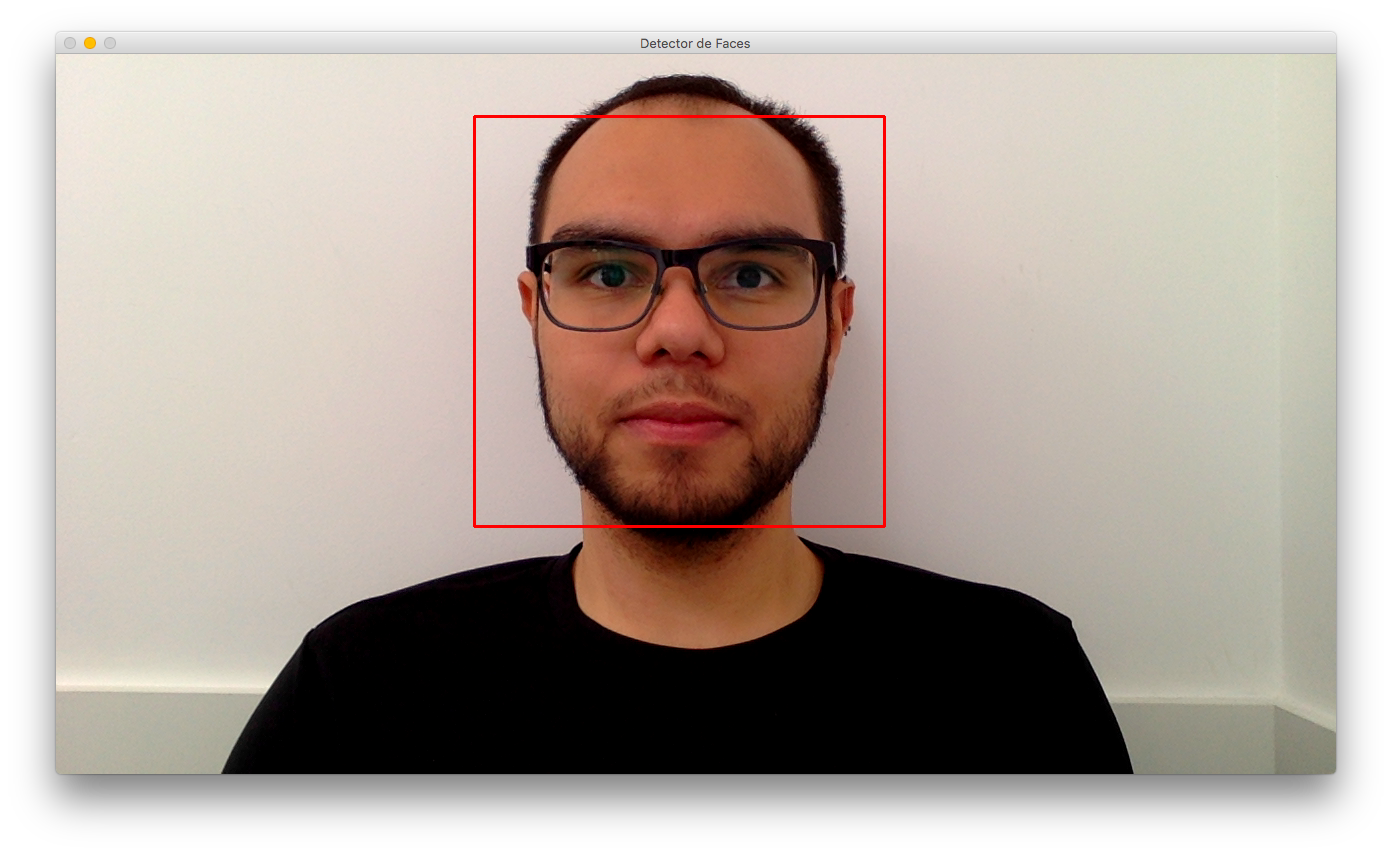
\includegraphics[width=0.4\linewidth]{imagens/detector_facial.png}}
    \end{center}
\end{figure}

\begin{figure}[htbp]
    \caption{Teste do classificador em cascata com imagens da Labeled Faces in the Wild}
    \label{fig:detector_facial_lfw}
    \begin{center}
        {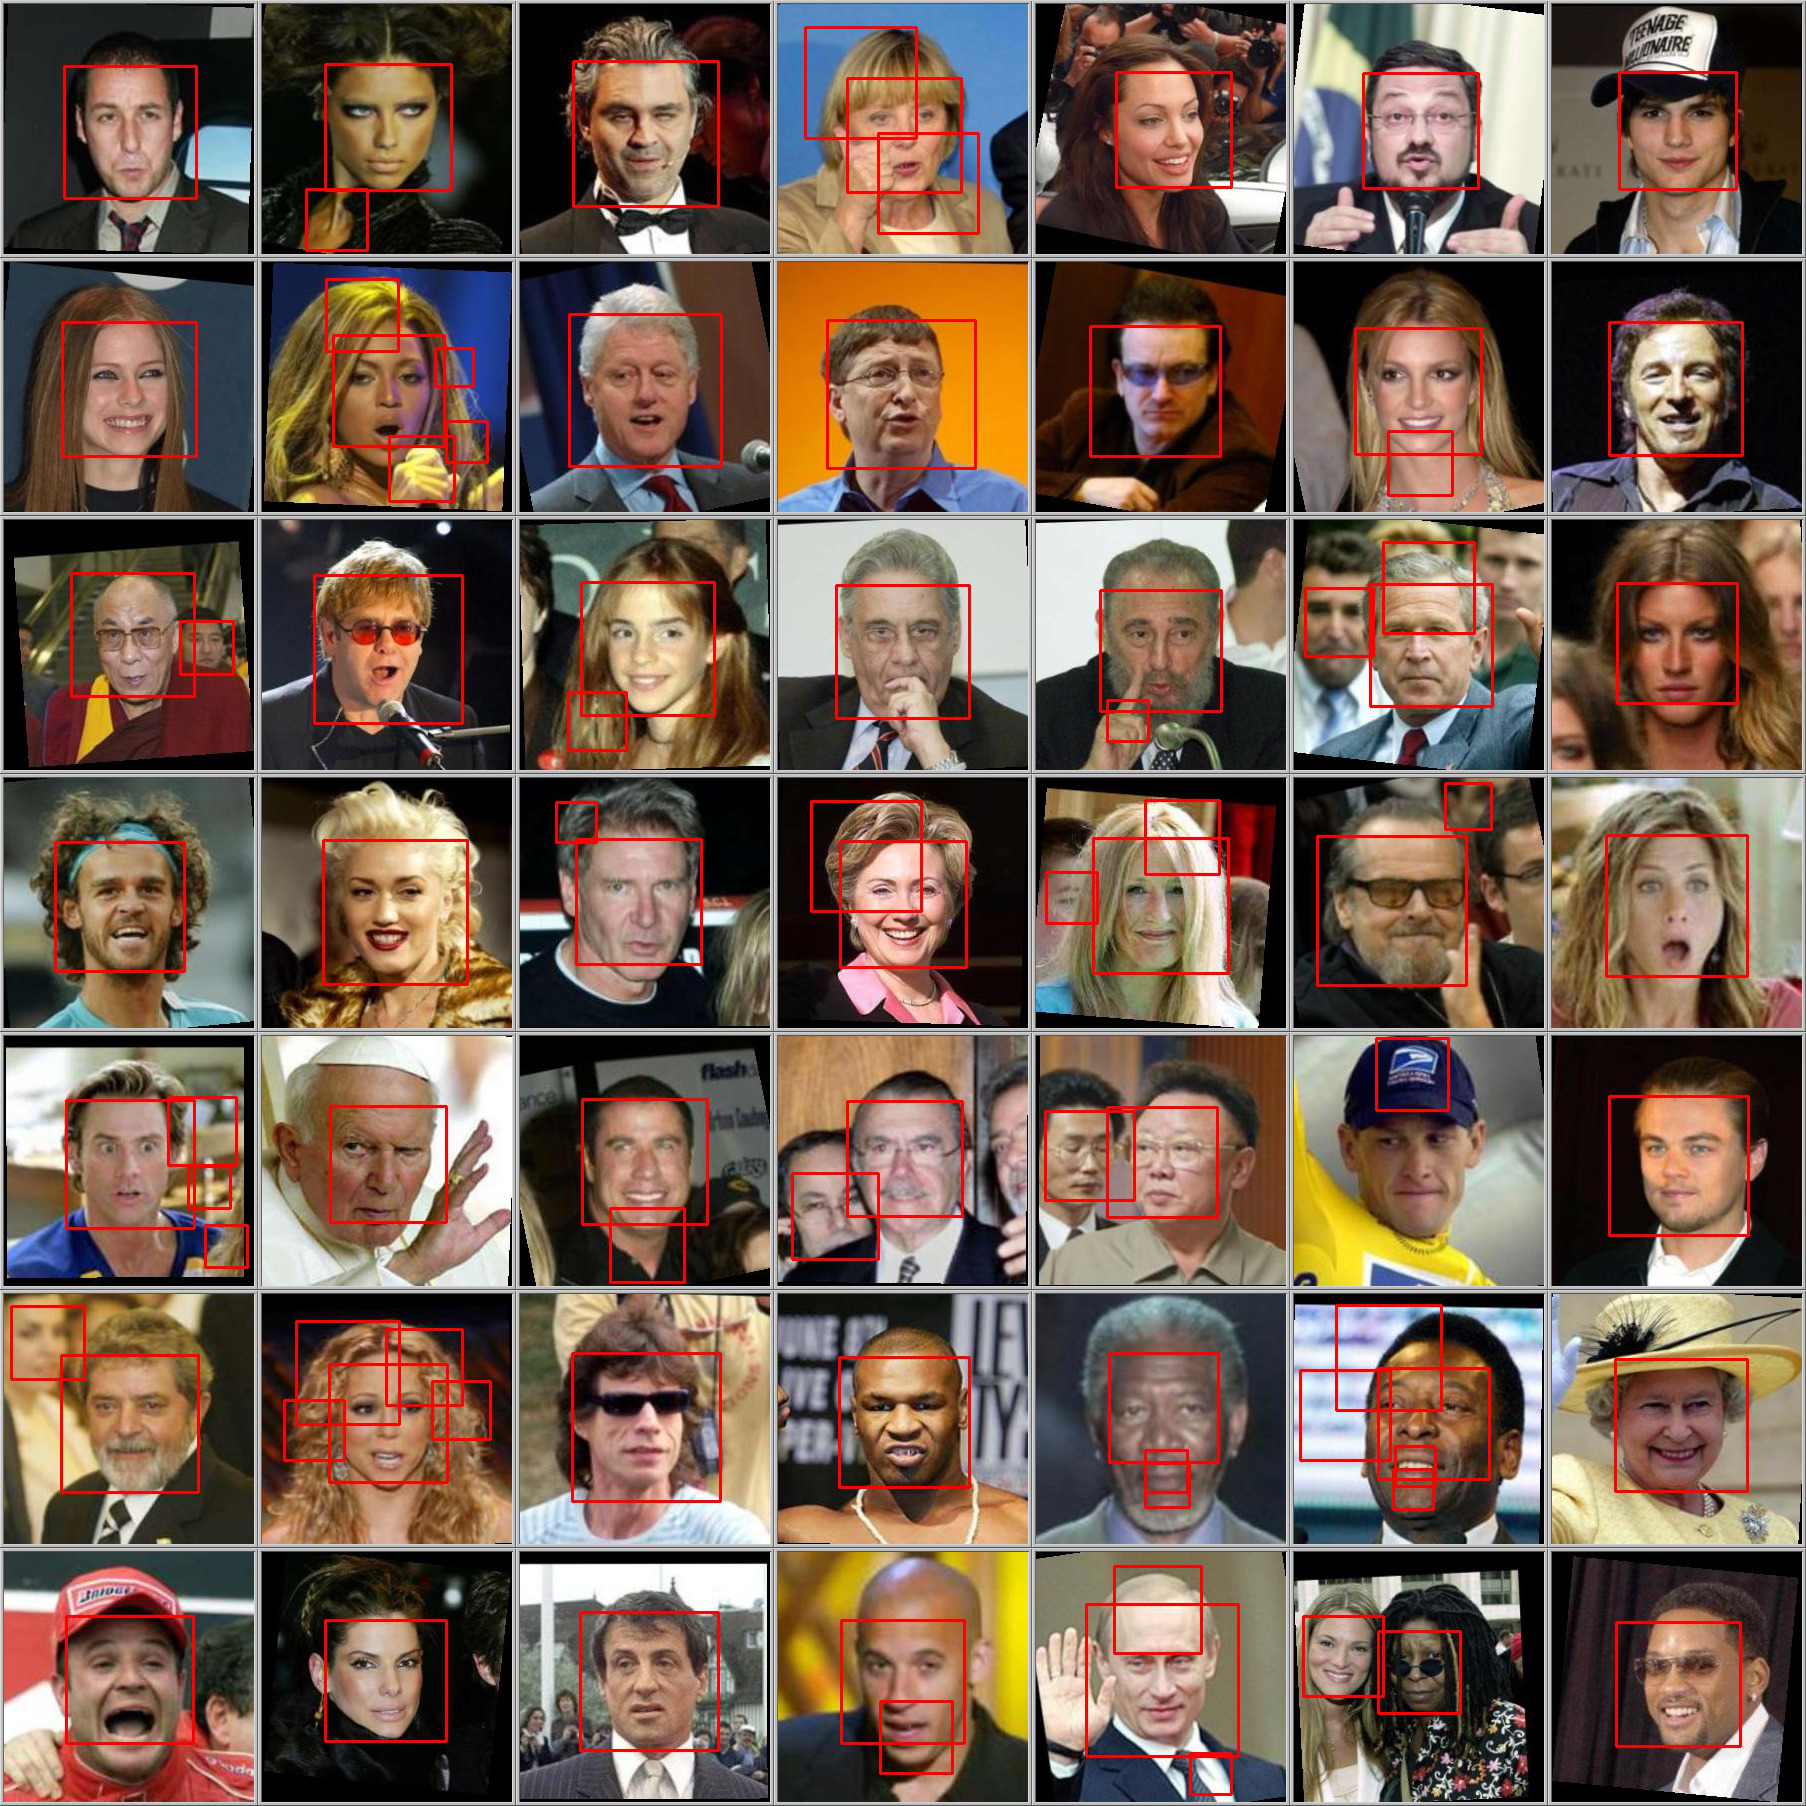
\includegraphics[width=0.99\linewidth]{imagens/detector_facial_lfw.jpg}}
    \end{center}
\end{figure}